نرخ نمونه‌برداری و هارمونیک‌های سیگنال:
\begin{flalign*}
    f_s &= \frac{1}{T_s} = \frac{1}{25\,\mu s} = 40\,\text{\lr{kHz}} \\
    x(t) &= \sum_{k=1}^{7}\cos(2\pi k f_\circ t),\quad f_\circ = 11\,\text{\lr{kHz}} \\
    kf_\circ &\in \{11,\,22,\,33,\,44,\,55,\,66,\,77\}\ \text{\lr{kHz}} &&
\end{flalign*}
هر مؤلفه در $kf_\circ$ پس از نمونه‌برداری تکرارهای طیفی در $kf_\circ + n f_s$ تولید می‌کند ($n \in \mathbb{Z}$). فیلتر پایین‌گذر تنها تکرارهایی با $|f|<16\,\text{\lr{kHz}}$ را عبور می‌دهد؛ نزدیک‌ترین \lr{alias} هر هارمونیک به باند پایه:
\begin{flalign*}
    11 &\to 11 \\
    22 &\to |22-40| = 18 \\
    33 &\to |33-40| = 7 \\
    44 &\to |44-40| = 4 \\
    55 &\to |55-40| = 15 \\
    66 &\to |66-80| = 14 \\
    77 &\to |77-80| = 3 &&
\end{flalign*}
بنابراین مؤلفهٔ $22$ (با alias در $18\,\text{\lr{kHz}}$) حذف می‌شود و بقیه عبور می‌کنند. هر تکرار دامنهٔ $\tfrac12$ دارد و نمونه‌بردار ضربه ضریب $f_s=\tfrac{1}{T_s}$ به طیف اعمال می‌کند:
\begin{flalign*}
    y(t) = f_s\Big[&\cos(2\pi\!\cdot\!3000\,t) + \cos(2\pi\!\cdot\!4000\,t) + \cos(2\pi\!\cdot\!7000\,t) \\
    +\,&\cos(2\pi\!\cdot\!11000\,t) + \cos(2\pi\!\cdot\!14000\,t) + \cos(2\pi\!\cdot\!15000\,t)\Big] &&
\end{flalign*}
تبدیل فوریه‌اش زوج‌ضربه‌هایی به ارتفاع $\tfrac{f_s}{2}$ در $\pm 3,\pm 4,\pm 7,\pm 11,\pm 14,\pm 15$ کیلوهرتز است:
\begin{flalign*}
    Y(f) = \frac{f_s}{2}\!\!\sum_{f_i \in \{3,4,7,11,14,15\}}\!\!\big[\delta(f-f_i) + \delta(f+f_i)\big]\ (\text{\lr{kHz}}) &&
\end{flalign*}

\begin{center}
\begin{tikzpicture}[>=stealth]
    \draw[->] (-8.2,0) -- (8.2,0) node[below right] {$f\,(\text{\lr{kHz}})$};
    \draw[->] (0,-0.3) -- (0,3) node[left] {$Y(f)$};
    \foreach \f in {-15,-14,-11,-7,-4,-3,3,4,7,11,14,15}{
        \draw[->,thick] (\f*0.5,0) -- (\f*0.5,2.2);
    }
    \foreach \f in {-15,-11,-7,-4,3,7,11,15}{
        \node[below,font=\scriptsize] at (\f*0.5,0) {$\f$};
    }
    \node[below left,font=\scriptsize] at (-14*0.5,0) {$-14$};
    \node[below right,font=\scriptsize] at (-3*0.5,0) {$-3$};
    \node[below,font=\scriptsize] at (4*0.5,-0.18) {$4$};
    \node[below,font=\scriptsize] at (14*0.5,0) {$14$};
    \node[right,font=\scriptsize] at (0.15,2.2) {$\dfrac{f_s}{2}$};
    \draw[dashed] (0,2.2) -- (15*0.5,2.2);
\end{tikzpicture}
\end{center}